\chapter{Validación experimental}\label{cap:validacion}

En este capítulo se muestran los resultados de la validación experimental de los objetivos expuestos en el capítulo \ref{cap:planificación}. Se explicarán detalladamente los procedimientos seguidos para el desarrollo de las tres aplicaciones robóticas de ejemplo.

\section{Procedimiento experimental y verificación de funcionalidad}

El procedimiento seguido para la validación experimental consiste en el desarrollo de las tres aplicaciones roboóticas de ejemplo utilizando exclusivamente BT Studio y usando el entorno de ejecución integrado. El proceso de creación de las aplicaciones robóticas es el mismo para todas ellas y este puede ser visto en el siguiente video: \url{https://youtu.be/0kK68lDe_Vo}.

Estas aplicaciones muestran el correcto funcionamiento de las siguientes funcionalidades de BT Studio creadas a lo largo de este TFG:

\begin{itemize}

    \item Acceso desde cualquier navegador tras la instalación en local de BT Studio, desde el contenedor de docker de BT Studio \footnote{\url{https://hub.docker.com/repository/docker/jderobot/bt-studio}} o desde la plataforma web de Unibotics usando el Robotics Backend. 

    \item Mecanismo para la gestión y navegación entre distintos proyectos robóticos. Cada proyecto almacena una sección donde se guardan el conjunto de acciones y árboles de comportamiento, y otra donde están los universos pertenecientes al mismo. 

    \item Mecanismo para la gestión y navegación entre distintos universos. Estos pueden ser los que vienen predefinidos en el Robotics Backend o personalizados. 
    
    \item Edición de ficheros Python para la programación acciones de un árbol de comportamiento. Además, si está conectado a un contenedor docker que contiene el Robotics Backend, como el contenedor de BT Studio, se le añade la funcionalidad de autocompletado, resaltado de sintaxis y formateo de  código en los ficheros de Python. 

    \item Creación de árboles de comportamiento mediante un editor visual basado en bloques (ya estaba en la versión de partida de BT Studio). Permite la creación de BT compatibles con el estándar definido en BT.cpp, el uso de acciones definidas por el usuario y su personalización.

    \item Integración con el Robotics Backend para la ejecución de las aplicaciones programadas por los usuarios. 
    
    \item Mecanismos para el control y visualización de la ejecución de las aplicaciones desde el navegador, así como la monitorización del estado de los árboles de comportamiento. 
    
\end{itemize}

Se desarrollaron tres aplicaciones robóticas ilustrativas con la versión final de BTStudio
desarrollada en este TFG: \textit{Laser Bump and Go}, \textit{Follow Person} y \textit{RoboCup Receptionist}. Las dos primeras fueron mejoradas a partir de las versiones existentes, mientras que la última fue creada enteramente en la versión offline de BT Studio desarrollada. Los videos fueron grabados en la versión offline, pero han sido replicados en el despliegue D1 de Unibotics y pueden ser reproducidos en el despliegue de producción de D3 de Unibotics.

\section{Aplicación: Laser Bump and Go}

Esta aplicación está basada en la disponible en la versión 0.3 de BT Studio, que consistía en que el robot vaya en línea recta hasta que encuentra un obstáculo y gira. Para la detección de obstáculos se usa un sensor láser a bordo del robot que es el turtlebot2.

También se muestra la composición de árboles de comportamiento que fue añadida por un proyecto del GSOC\footnote{\url{https://theroboticsclub.github.io/gsoc2024-Oscar_Martinez/}}.

\subsection{Resumen}

\begin{itemize}
    \item \textbf{Código para consulta:} \url{https://github.com/JdeRobot/bt-studio/tree/main/backend/filesystem/composition_demo}
    \item \textbf{Simulador:} Gazebo Classic.
    \item \textbf{Robot:} TurtleBot2.
    \item \textbf{Universo:} Hospital (Follow Person) del Robotics Backend llamado \textit{default} en BT Studio.
    \item \textbf{Sensores:} LIDAR 2D.
    \item \textbf{Sentido de ejecución:} de arriba hacia abajo. 
\end{itemize}

\subsection{Implementación en BT Studio}

\subsubsection{Listado de acciones}
\begin{itemize}
    \item \textbf{Forward:} obtiene la velocidad lineal deseada a través del puerto de entrada \textit{lin\_speed} y la publica a través del topic \textit{/cmd\_vel}. Cuando le llega un tick devuelve \textit{Running}. 
    \item \textbf{Turn:} obtiene la velocidad angular deseada a través del puerto de entrada \textit{ang\_speed} y la publica a través del topic \textit{/cmd\_vel}. Cuando le llega un tick devuelve \textit{Running}. 
    \item \textbf{CheckObstacle:} se suscribe al topic \textit{/scan} donde se publican las medidas del láser. Cuando le llega un tick, si las medidas del láser dentro de la amplitud deseada que obtiene a través del puerto de entrada \textit{amplitude} son menores que la distancia mínima indicada en el puerto de entrada \textit{obs\_dist} devuelve \textit{Success} y en caso contrario, \textit{Failure}. 
\end{itemize}

\subsubsection{Árbol de comportamiento}
Al estar formado por composición de árboles de comportamiento hay dos subárboles y un árbol principal.

\begin{itemize}
    \item Árbol de comportamiento principal: tiene un subárbol dentro llamado \textit{AvoidObstacle}. Figura \ref{fig:lbg-1}.
    \begin{figure}[H]
        \centering
        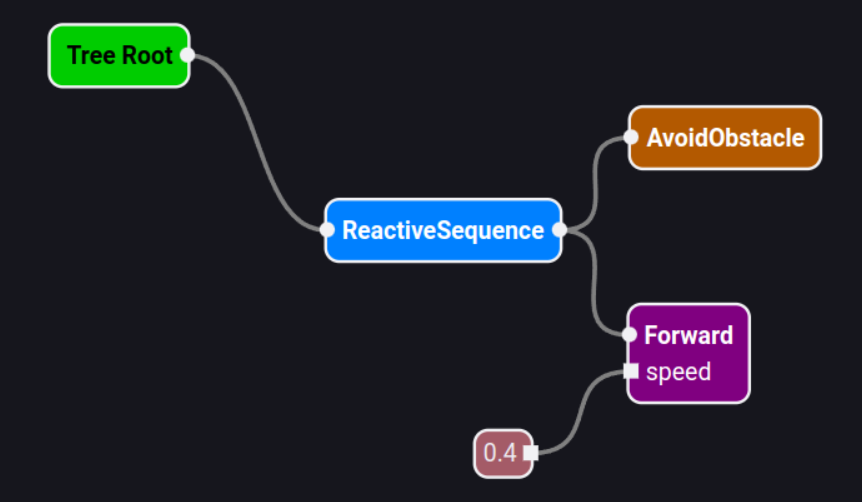
\includegraphics[width=0.65\textwidth]{figures/validation/BumpAndGo_1.png}
        \caption{Árbol de comportamiento principal de Laser Bump and Go}
        \label{fig:lbg-1}
    \end{figure}
    \item Subárbol de comportamiento \textit{AvoidObstacle}: tiene un subárbol dentro llamado \textit{ObstacleDetection}. Figura \ref{fig:lbg-2}.
    \begin{figure}[H]
        \centering
        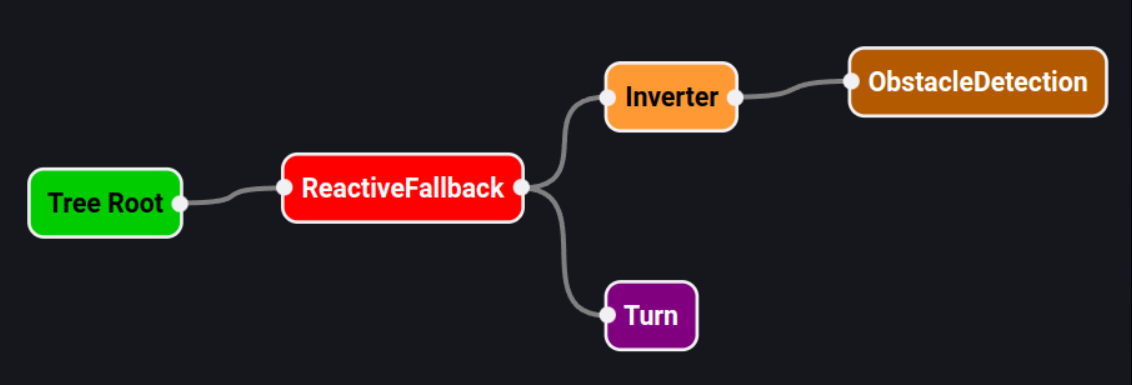
\includegraphics[width=0.65\textwidth]{figures/validation/BumpAndGo_2.png}
        \caption{Subárbol de comportamiento \textit{AvoidObstacle} de Laser Bump and Go}
        \label{fig:lbg-2}
    \end{figure}
    \item Subárbol de comportamiento \textit{ObstacleDetection}. Figura \ref{fig:lbg-3}.
    \begin{figure}[H]
        \centering
        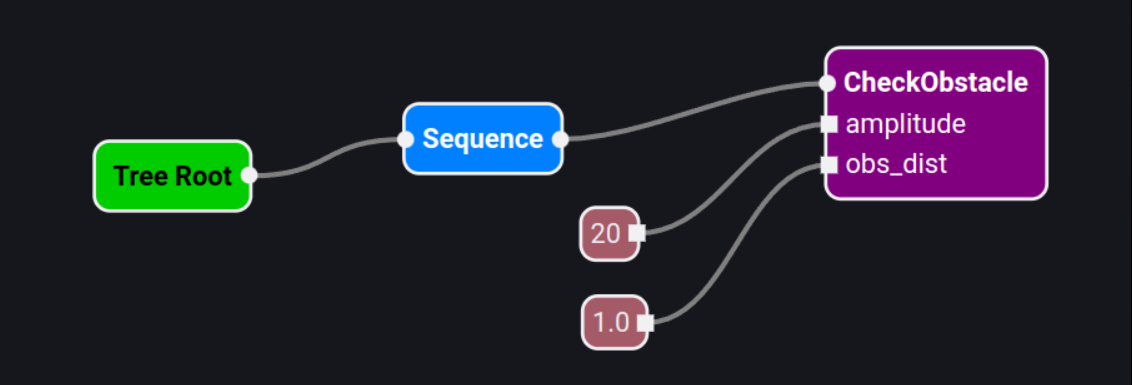
\includegraphics[width=0.65\textwidth]{figures/validation/BumpAndGo_3.png}
        \caption{Subárbol de comportamiento \textit{ObstacleDetection} de Laser Bump and Go}
        \label{fig:lbg-3}
    \end{figure}
\end{itemize}

\subsubsection{Flujo de ejecución}

Como el sentido de ejecución es de arriba hacia abajo, lo primero que se ejecuta es el \textit{ReactiveSequence}, que hace \textit{tick} al subárbol \textit{AvoidObstacle}, donde se ejecuta el \textit{ReactiveFallback}. Dentro del \textit{ReactiveFallback} se hace tick al subárbol \textit{ObstacleDetection} que ejecuta \textit{CheckObstacle}. Si este detecta un obstáculo devolverá \textit{Success}, pero al pasar por el \textit{Inverter} se convierte en \textit{Failure}, lo que hace que se pase a ejecutar \textit{Turn}, que reiniciará el \textit{ReactiveFallback} debido a que siempre devuelve \textit{Running}.

En caso de que \textit{CheckObstacle} no detecte un obstáculo, devolverá \textit{Failure}, que al pasar por el \textit{Inverter} se convierte en \textit{Success}. Esto producirá que se termine la ejecución del \textit{ReactiveFallback} y se ejecute \textit{Forward}. Como este siempre devuelve \textit{Running}, se reiniciará la ejecución de la \textit{ReactiveSequence}. 

\subsection{Ejecución típica}

El vídeo demostrativo de esta aplicación se puede encontrar en el siguiente enlace: \url{https://www.youtube.com/watch?v=luxoZLU-Y8g}.

\begin{figure}[H]
    \centering
    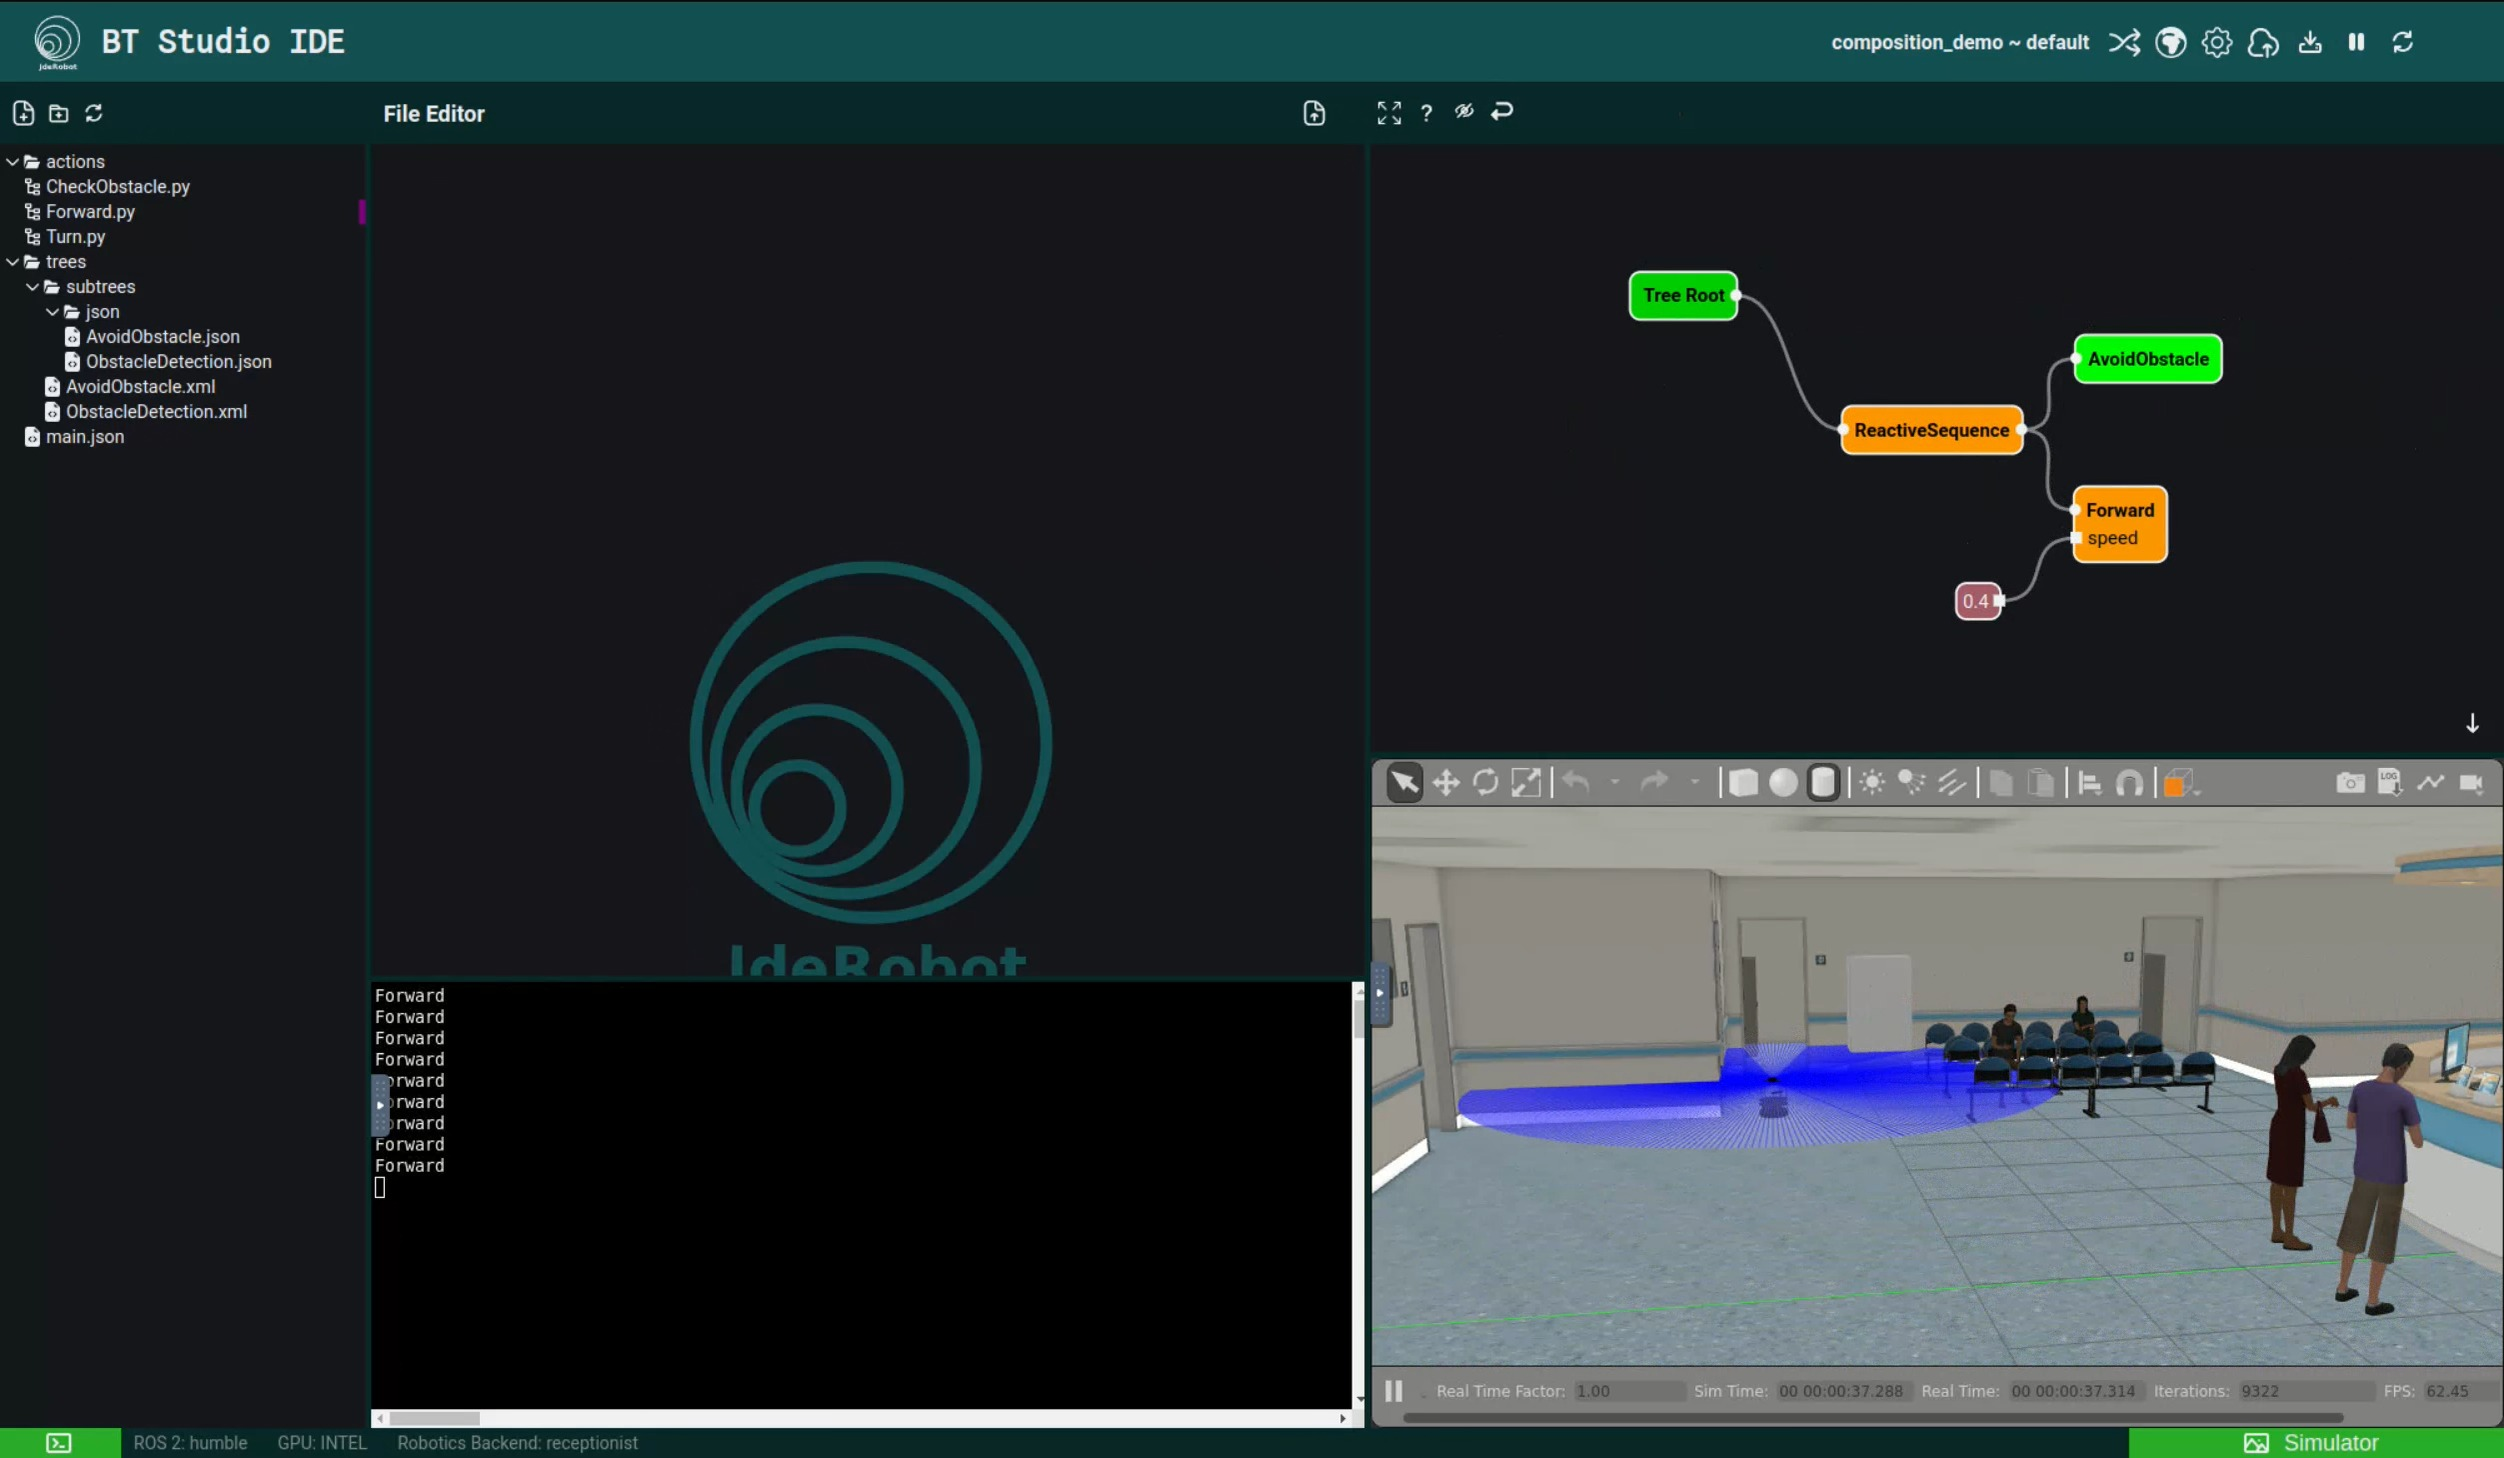
\includegraphics[width=0.7\textwidth]{figures/validation/bump-teaser.jpg}
    \caption{Aplicación Laser Bump and Go en funcionamiento}
    \label{fig:ejemplo}
\end{figure}

\noindent Los momentos más destacados de la ejecución de esa aplicación son:

\begin{itemize}
    \item \texttt{0:07}: comienza la ejecución. Como \textit{CheckObstacle} no detecta un obstáculo, se sale del callback y se ejecuta \textit{Forward}. Tras ello se reiniciará la secuencia. Mientras esto ocurra, el robot avanza hacia delante de manera constante.
    
    En el monitor de ejecución como \textit{CheckObstacle} no detecta un obstáculo, el subárbol \textit{AvoidObstacle} devuelve \textit{Success}, mientras que \textit{Forward} devuelve \textit{Running}.
    \item \texttt{0:12}: se entra en el subárbol \textit{AvoidObstacle} dentro del monitor de ejecución y se muestra que el subárbol \textit{ObstacleDetection} devuelve \textit{Failure} al no detectar obstáculos, pero está invertido por el \textit{Inverter}. Mientras \textit{Turn} está en gris porque no se encuentra en ejecución.
    \item \texttt{0:26}: \textit{CheckObstacle} detecta un obstáculo, por lo que se ejecutará el siguiente componente del \textit{callback}, \textit{Turn}. Esto produce que mientras se detecte un obstáculo, el robot gire de manera constante.

    En el monitor de ejecución se muestra cómo \textit{Turn} pasa a ejecutarse devolviendo \textit{Running}.
    \item \texttt{0:31}: \textit{CheckObstacle} ya no detecta un obstáculo, por lo que se deja de ejecutar \textit{Turn} y se vuelve a ejecutar \textit{Forward}.
    \item \texttt{0:35}: se vuelve a detectar un obstáculo. Se ejecuta \textit{Turn} de nuevo.

    En el monitor de ejecución se muestra cómo \textit{Forward} pasa a no ejecutarse. 
\end{itemize}

Este comportamiento se repite en el resto del vídeo. 

\section{Aplicación: Visual Follow Person}

Esta aplicación está basada en la anterior que había disponible en la versión 0.3 de BT Studio, que consistía en que el robot siga a una persona. Para la detección de la misma se utiliza un filtro de color sobre la imagen de la cámara y se comanda al robot con las velocidades angulares y lineales adecuadas para mantener a la persona lo más centrada en la imagen posible.

\subsection{Resumen}

\begin{itemize}
    \item \textbf{Código para consulta:} \url{https://github.com/JdeRobot/bt-studio/tree/main/backend/filesystem/visual_follow_person}
    \item \textbf{Simulador:} Gazebo Classic.
    \item \textbf{Robot:} TurtleBot2.
    \item \textbf{Universo:} Hospital (Follow Person) del Robotics Backend llamado \textit{default} en BT Studio.
    \item \textbf{Sensores:} Cámara RGB.
    \item \textbf{Sentido de ejecución:} de abajo hacia arriba. 
\end{itemize}

\subsection{Implementación en BT Studio}

\subsubsection{Listado de acciones}
\begin{itemize}
    \item \textbf{DetectPerson:} se suscribe al topic \textit{/depth\_camera/image\_raw} donde se publican las imágenes de la cámara. Cuando llega un tick, aplica un filtro de color verde e intenta calcular el centroide de la imagen filtrada. Si este existe, se está detectando a la persona y se publica el valor de su componente X en el puerto de salida \textit{person\_pos}. Si se ha detectado a la persona se devuelve \textit{Success}, en caso contrario \textit{Failure}. 
    \item \textbf{Turn:} gira a una velocidad angular indicada en el puerto de entrada \textit{ang\_speed}. Cuando le llega un tick devuelve \textit{Running}. 
    \item \textbf{Move:} recibe por el puerto de entrada \textit{person\_pos} la posición de la persona en el eje X de la imagen y por el puerto de entrada \textit{image\_x\_center} el centro en X de la imagen. Con esto calcula el error de seguimiento como la diferencia entre el centro de la imagen y la posición de la persona. Aplicando un controlador proporcional, calcula la velocidad lineal y angular adecuada. Una vez calculada, la publica a través del topic \textit{/cmd\_vel}. Cuando le llega un tick devuelve \textit{Running}. 
\end{itemize}

\subsubsection{Árbol de comportamiento}
\begin{figure}[H]
    \centering
    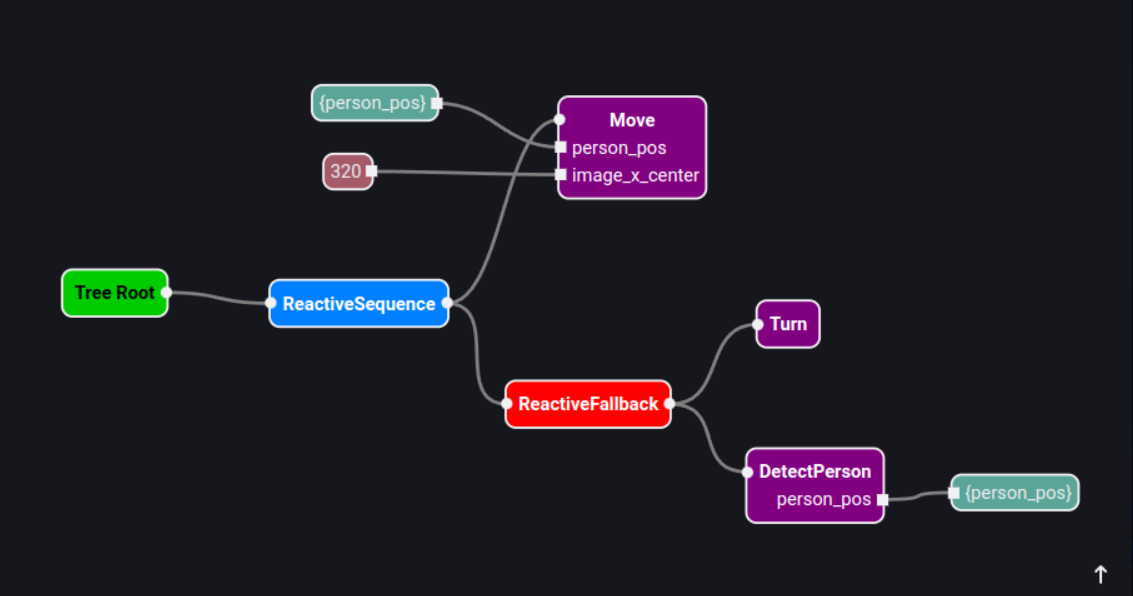
\includegraphics[width=0.7\textwidth]{figures/validation/FollowPerson_1.png}
    \caption{Árbol de comportamiento de Visual Follow Person}
    \label{fig:ejemplo}
\end{figure}

\subsubsection{Flujo de ejecución}

Como el sentido de ejecución es de abajo hacia arriba, lo primero en ejecutarse es el \textit{ReactiveFallback}, que hace \textit{tick} a \textit{DetectPerson}. Si este detecta a una persona, devolverá \textit{Success}, lo que termina la ejecución del \textit{ReactiveFallback}. En el caso opuesto se hará \textit{tick} a \textit{Turn} que como siempre devuelve \textit{Running} reinicia el \textit{ReactiveFallback}.

Cuando se detecta a una persona se termina el \textit{ReactiveFallback} y empieza a ejecutarse \textit{Move}, y como este también devuelve siempre, \textit{Running} reiniciará el \textit{ReactiveSequence}.

\subsection{Ejecución típica}

El vídeo demostrativo de esta aplicación se puede encontrar en el siguiente enlace: \url{https://www.youtube.com/watch?v=q_K0pl-IoFA}. 

\begin{figure}[H]
    \centering
    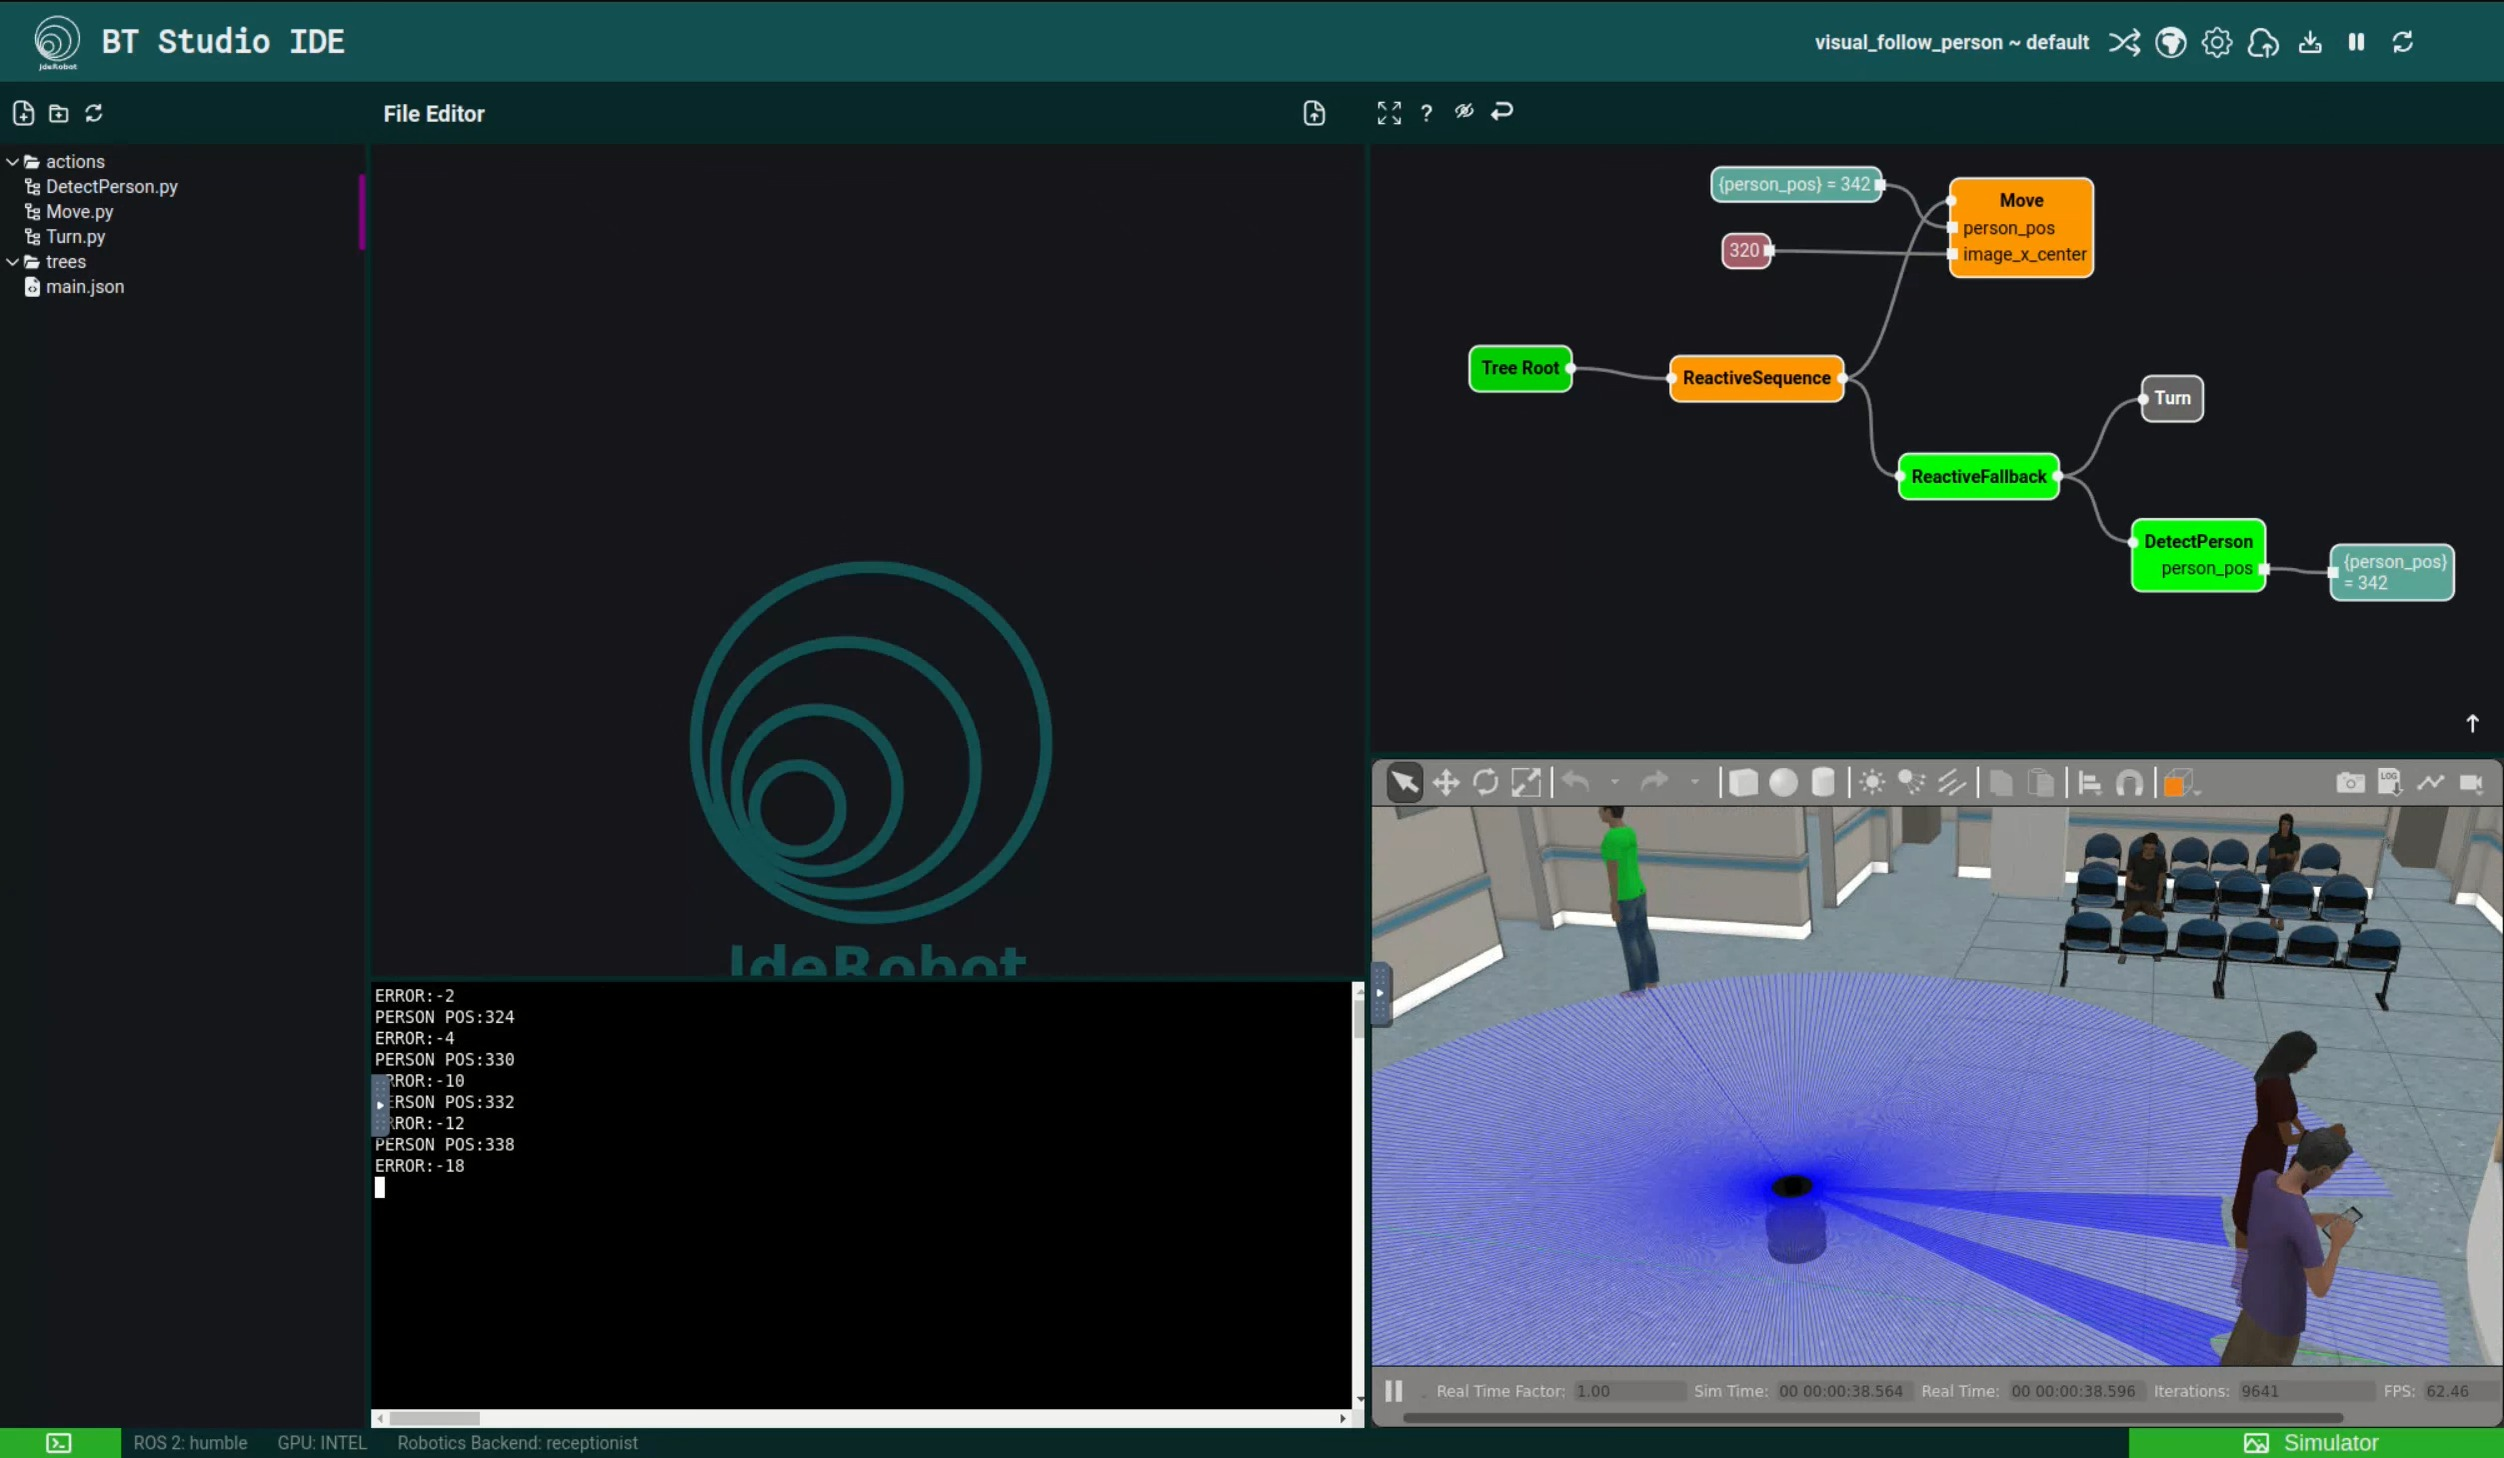
\includegraphics[width=0.7\textwidth]{figures/validation/followPerson-teaser.jpg}
    \caption{Aplicación Visual Follow Person en funcionamiento}
    \label{fig:ejemplo}
\end{figure}


\noindent A lo largo del video se muestra cómo el monitor de ejecución se actualiza para mostrar en tiempo real el contenido de la etiqueta del \textit{blackboard}, \textit{\{person\_pos\}}.

\noindent Los momentos más destacados de la ejecución de la aplicación son:

\begin{itemize}
    \item \texttt{0:06}: comienza la ejecución. \textit{DetectPerson} consigue identificar una persona en la imagen, lo que causa que se salga del \textit{ReactiveFallback} y se ejecute \textit{Move}. Este calcula las velocidades necesarias para mantener a la persona en el centro de la imagen. \textit{DetectPerson} mantiene actualizada esta información en cada iteración. 

    En el monitor de ejecución como \textit{DetectPerson} detecta a una persona devuelve \textit{Success}, lo que hace que se ejecute \textit{Move} que devuelve \textit{Running}. Como la detección de la persona hace que se acabe el \textit{ReactiveFallback}, \textit{Turn} se muestra en gris porque no se ejecuta.

    \item \texttt{0:23}: al acercarse demasiado a la persona se pierde la detección de la misma, por lo que \textit{DetectPerson} devuelve \textit{Failure}. Debido a esto se empieza a ejecutar \textit{Turn}. 

    En el monitor de ejecución como \textit{Turn} devuelve \textit{Running} se resetean tanto el \textit{ReactiveFallback} como el \textit{ReactiveSequence}, lo que hace que \textit{Move} se muestre en gris porque no se ejecuta. También se muestra que al no detectar a una persona el contenido de la etiqueta del \textit{blackboard}, \textit{\{person\_pos\}}, pasa a ser -1.
\end{itemize}

\section{Aplicación: RoboCup Receptionist}

Esta aplicación está basada en una versión simplificada del desafío de Receptionist de la Robocup Home 2022 \footnote{\url{https://athome.robocup.org/wp-content/uploads/2022_rulebook.pdf}}. Esta consiste en los siguientes pasos:
\begin{enumerate}
    \item El robot debe ir a la puerta de la casa a esperar a que una persona aparezca.
    \item Cuando haya una persona se le debe preguntar por su nombre.
    \item Se acompaña al invitado al salón donde se le presenta por su nombre y se le pregunta qué bebida prefiere.
    \item El robot navega hasta la cocina para pedir que se le entregue la bebida especificada por el invitado.
    \item El robot vuelve al salón y le entrega la bebida.
    \item Se repite desde el principio.
\end{enumerate}

Para la navegación del robot se usa el paquete de Nav2 y para la detección de la persona se usa el paquete de DarknetRos que contiene la red neuronal de Yolov4.

El objetivo de esta aplicación de ejemplo era demostrar la capacidad de BT Studio para crear aplicaciones más complejas que las dos anteriores y que usen paquetes externos habituales en la comunidad
robótica como Nav2.

\subsection{Resumen}

\begin{itemize}
    \item \textbf{Código para consulta:} \url{https://github.com/JdeRobot/bt-studio/tree/receptionist_demo/backend/filesystem/receptionist_demo}
    \item \textbf{Simulador:} Gazebo Harmonic.
    \item \textbf{Robot:} TurtleBot3.
    \item \textbf{Universo:} Receptionist Demo del Robotics Backend llamado \textit{receptionist} en BT Studio.
    \item \textbf{Sensores:} Cámara RGB, LIDAR 2D.
    \item \textbf{Sentido de ejecución:} de abajo hacia arriba. 
\end{itemize}

\subsection{Implementación en BT Studio}

\subsubsection{Listado de acciones}
\begin{itemize}
    \item \textbf{AskDrink:} pregunta usando el terminal qué bebida prefiere el invitado y guarda su respuesta en el puerto de salida \textit{drink}. Si la respuesta contiene más de un carácter devolverá \textit{Success}, en caso contrario devuelve \textit{Failure}. 
    \item \textbf{AskName:} pregunta usando el terminal por el nombre del invitado y guarda su respuesta en el puerto de salida \textit{person}. Si la respuesta contiene más de un carácter devolverá \textit{Success}, en caso contrario devuelve \textit{Failure}.
    \item \textbf{Greet:} saluda al invitado usando el nombre que obtiene del puerto de entrada \textit{person}. Siempre devuelve \textit{Success}.
    \item \textbf{Move:} al iniciarse se lanza la acción de Nav2 con el objetivo proveniente del puerto de entrada \textit{waypoint}. Devuelve \textit{Running} mientras que se está ejecutando, \textit{Success} cuando finaliza de forma correcta y \textit{Failure} si la navegación se encuentra con algún error.
    \item \textbf{OrderDrink:} pide la bebida especificada por el invitado que es obtenida del puerto de entrada \textit{drink}. Siempre devuelve \textit{Success}.
    \item \textbf{ServeDrink:} entrega la bebida especificada por el invitado, cuyo nombre viene del puerto de entrada \textit{person}, que es obtenida del puerto de entrada \textit{drink}. Siempre devuelve \textit{Success}.
    \item \textbf{SetDestination:} escribe el destino correcto en el puerto de salida \textit{waypoint} a partir del ID proveniente del puerto de entrada \textit{waypoint\_id}. El destino será usado en la acción de \textit{Move}. Siempre devuelve \textit{Success}.
    \item \textbf{WaitPerson:} espera hasta que YoloV4 detecta una persona en la imagen con un 99\% de precisión. Devuelve \textit{Running} mientras que está esperando y \textit{Success} cuando encuentra a una persona.
\end{itemize}

\subsubsection{Árbol de comportamiento}
\begin{figure}[H]
    \centering
    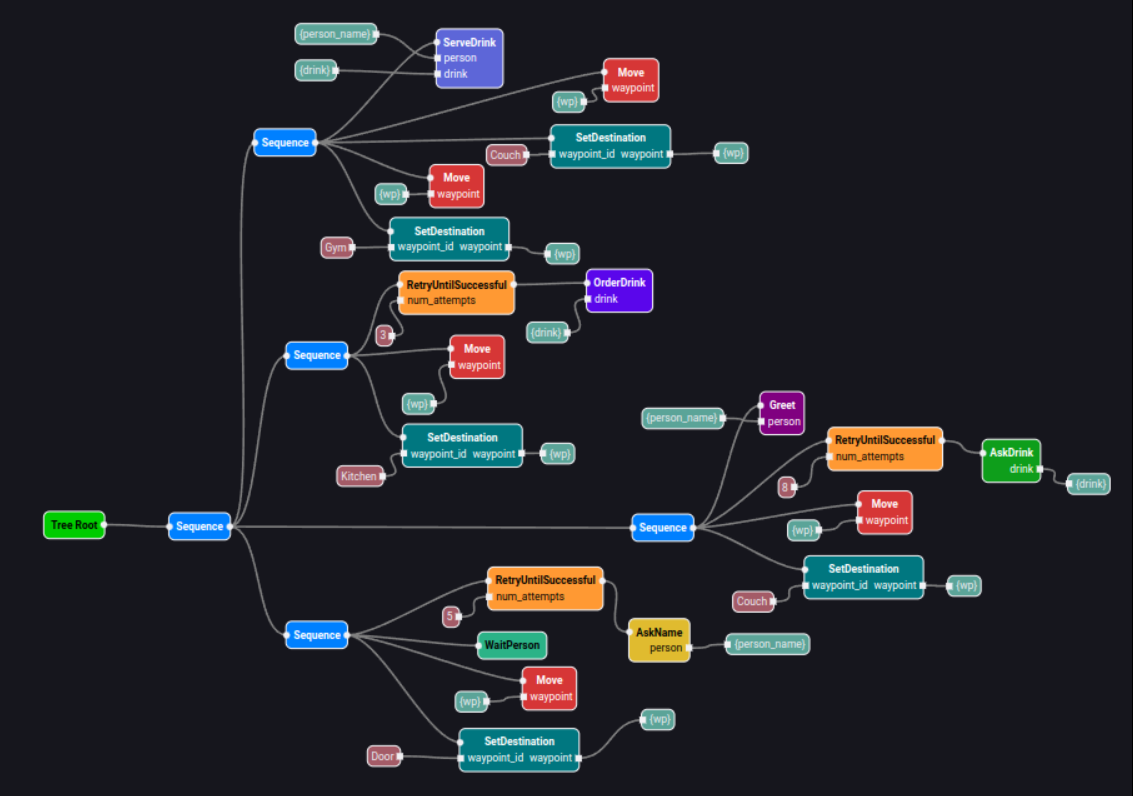
\includegraphics[width=0.7\textwidth]{figures/validation/Receptionist_1.png}
    \caption{Árbol de comportamiento de RoboCup Receptionist}
    \label{fig:ejemplo}
\end{figure}

\subsubsection{Flujo de ejecución}

Como el sentido de ejecución es de abajo hacia arriba, lo primero en ejecutarse es el \textit{Sequence} inferior, que hace \textit{tick} a \textit{SetDestination}. Al devolver este siempre \textit{Success}, se empezará a ejecutar \textit{Move} hasta que finalice la navegación de forma correcta. Si es así, se pasa a esperar a la persona en \textit{WaitPerson} y cuando se la detecte, se preguntará el nombre a la misma en \textit{AskName} hasta 5 veces si la respuesta es inválida, en caso de que la respuesta final sea inválida se reinicia todo desde el principio.

Al acabar la secuencia anterior se empieza a ejecutar el siguiente \textit{Sequence} donde las dos primeras acciones se realizan de la misma forma que anteriormente, solo variando el \textit{waypoint\_id}. Después de eso se pregunta hasta 5 veces por la bebida preferida del invitado en \textit{AskDrink}. Si la respuesta ha sido válida, se ejecuta a continuación la acción \textit{Greet} para presentar al invitado. 

La siguiente secuencia sigue usando las dos primeras acciones de los otros \textit{Sequence} variando el \textit{waypoint\_id}. Si la acción de \textit{Move} finaliza con \textit{Success} se pasa a ejecutar hasta 5 veces \textit{OrderDrink} para pedir la bebida del invitado.

Con esto se pasa a la última secuencia donde se ejecutan por partida doble las acciones de \textit{SetDestination} y \textit{Move} de igual manera que en las secuencias anteriores variando el \textit{waypoint\_id} para moverse primero a un punto intermedio y luego al salón. Si todo esto se realiza con \textit{Success} se llama a \textit{ServeDrink} donde se entrega la bebida al invitado.

Todo esto se repite indefinidamente.

\subsection{Ejecución típica}

El vídeo demostrativo de esta aplicación se puede encontrar en el siguiente enlace: \url{https://www.youtube.com/watch?v=2AuwqGPP8WQ}. 

\begin{figure}[H]
    \centering
    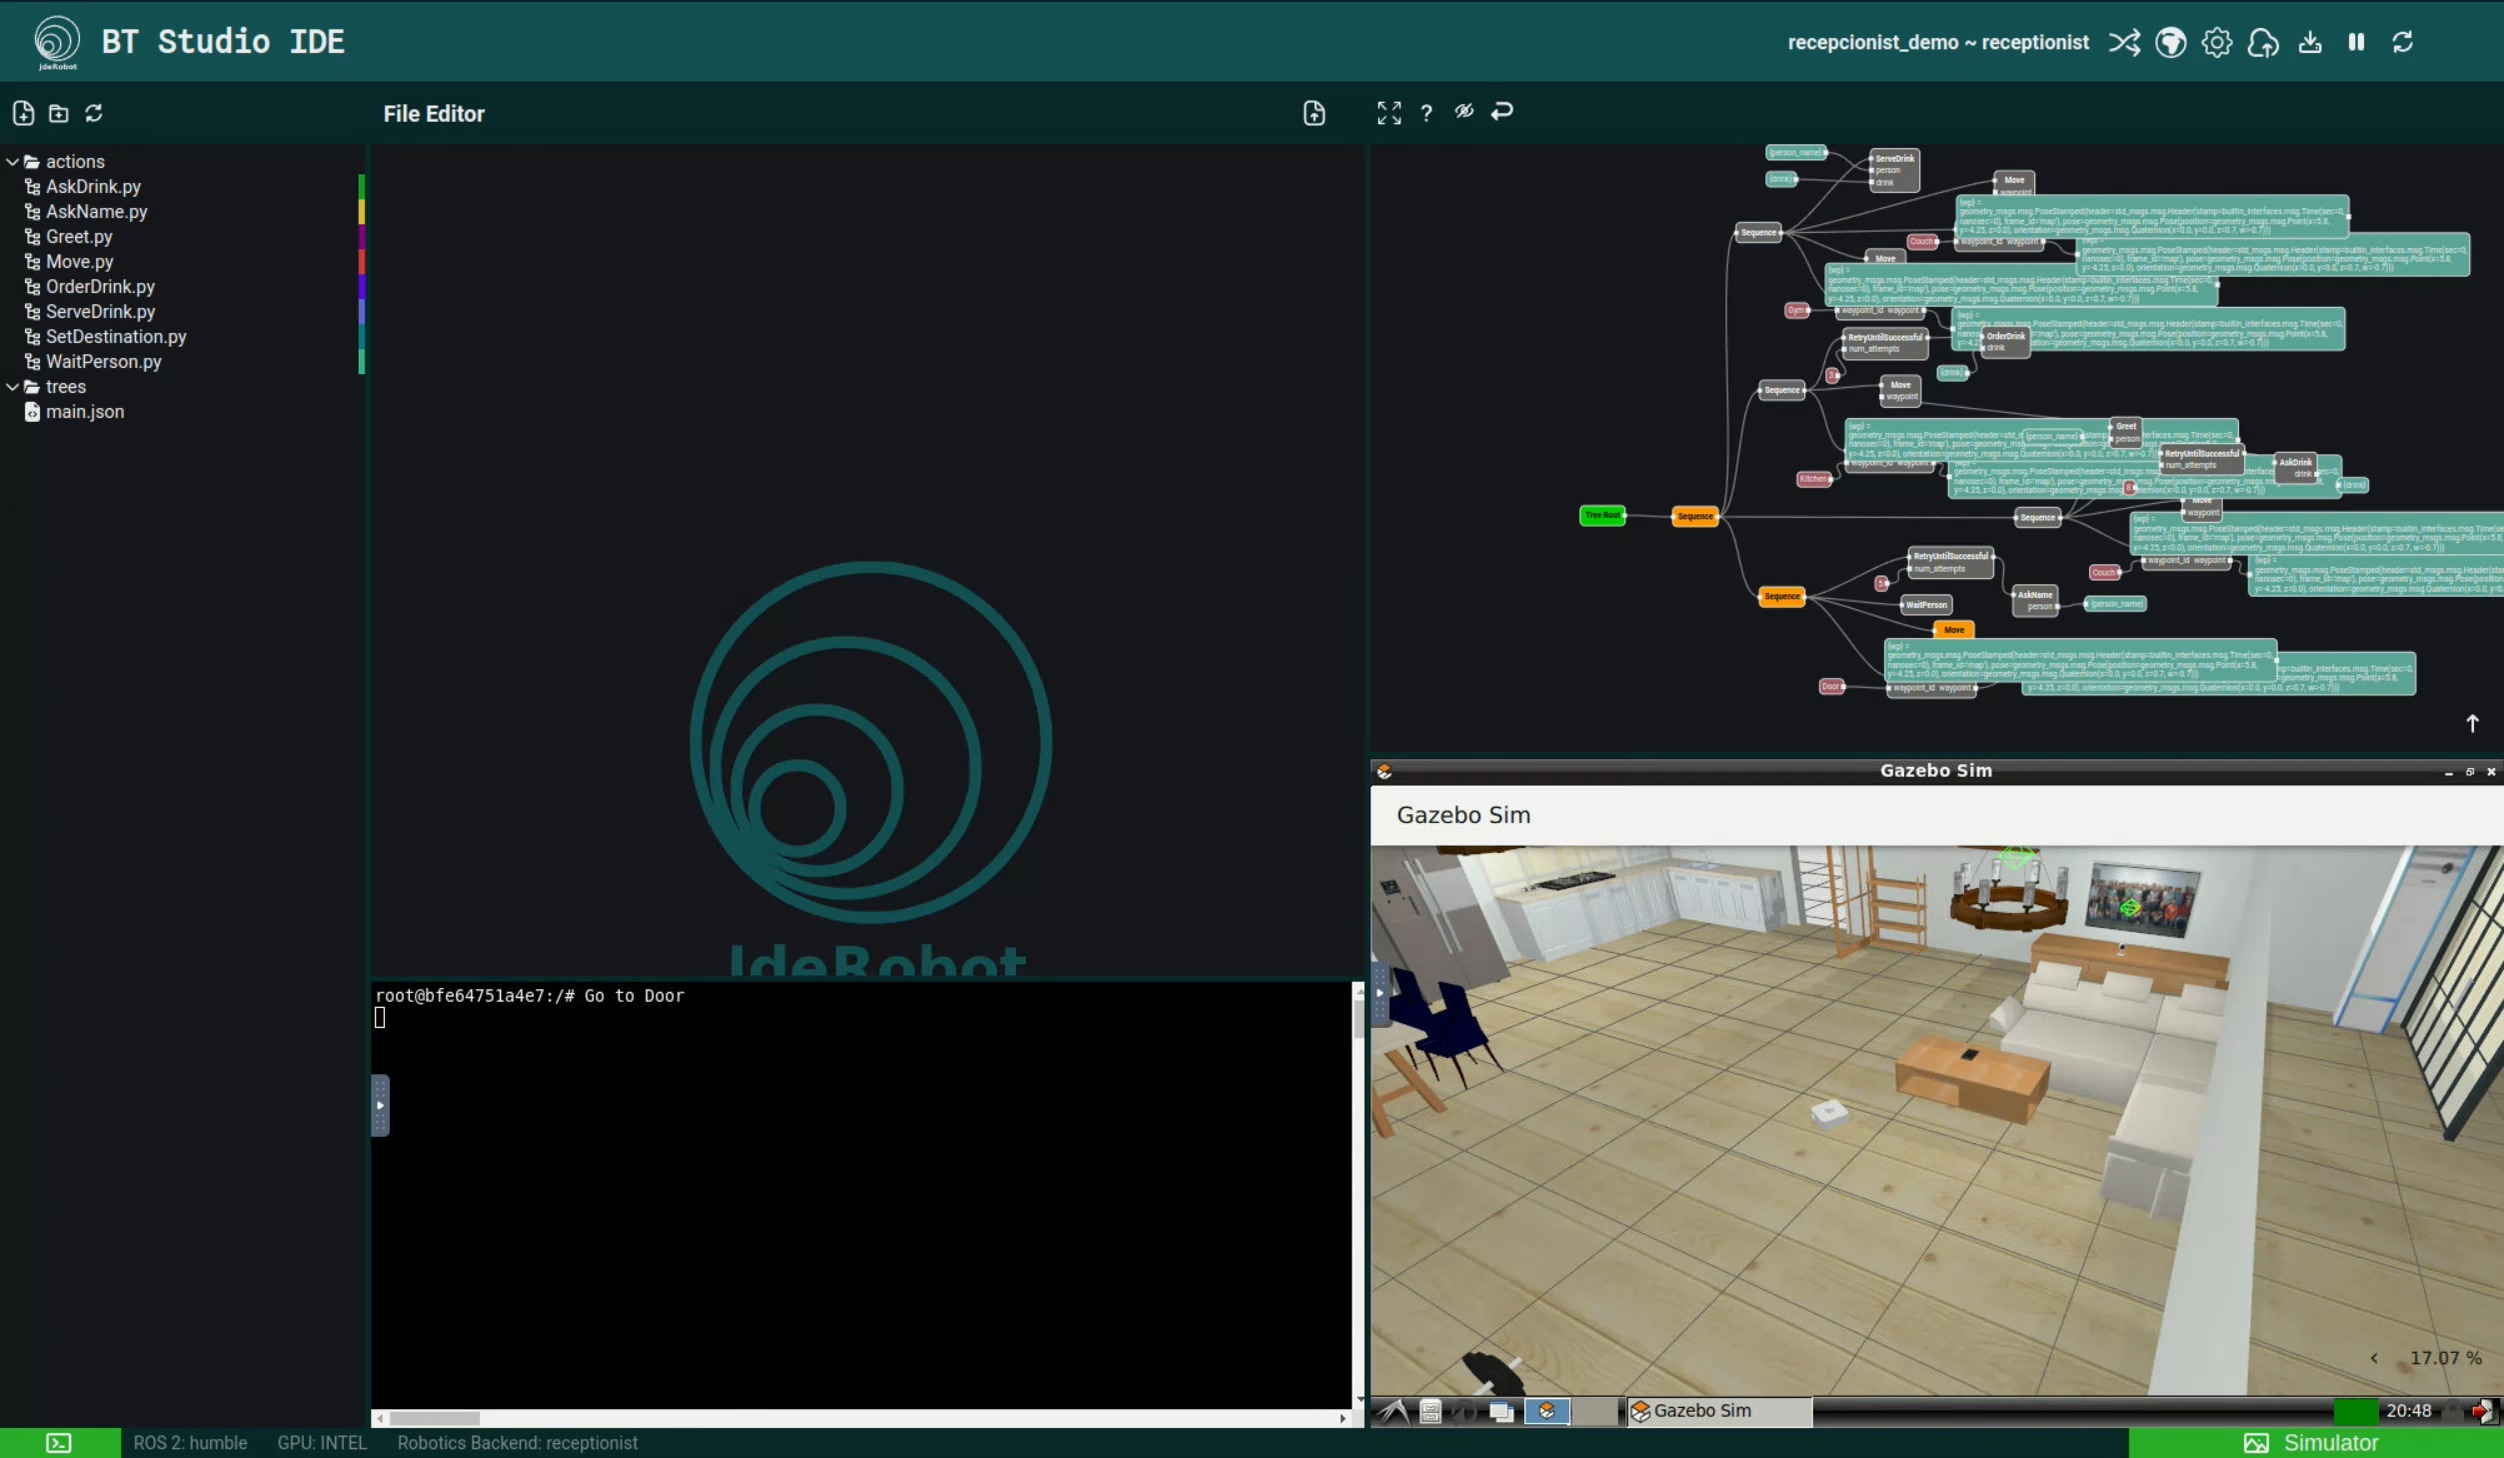
\includegraphics[width=0.7\textwidth]{figures/validation/receptionist-teaser.jpg}
    \caption{Aplicación RoboCup Receptionist en funcionamiento}
    \label{fig:ejemplo}
\end{figure}

\noindent A lo largo del video se muestra cómo el monitor de ejecución se actualiza para mostrar en tiempo real el contenido de las etiquetas del \textit{blackboard}, \textit{\{drink\}}, \textit{\{person\_name\}} y \textit{\{wp\}}.

\noindent Para no tener que controlar de forma manual a la persona, se le asigna una ruta cerca de la puerta para simular que llega, por lo que no tiene la capacidad de seguir al robot hasta los diferentes puntos como el salón.

\noindent Los momentos más destacados de la ejecución de la aplicación son:

\begin{itemize}
    \item \texttt{0:05}: comienza la ejecución.\textit{SetDestination} pone como destino en \textit{\{wp\}} la puerta y se empieza a ejecutar \textit{Move} usando Nav2 para ir a esa posición.

    En el monitor de ejecución se muestra cómo \textit{SetDestination} pone en \textit{\{wp\}} la posición de la puerta y cómo solo se ejecuta \textit{Move}, que devuelve \textit{Running}. 
    \item \texttt{0:23}: el robot llega a la puerta, espera en \textit{WaitPerson} hasta que detecta a una persona, es decir, devuelve \textit{Success}. Entonces, usando el terminal \textit{AskName} pregunta al invitado por su nombre y al contestar este de forma válida, el robot empieza a moverse hacia el salón. Esto ha sido gracias a que \textit{SetDestination} ha cambiado el valor de \textit{\{wp\}} y empieza a ejecutarse \textit{Move}.

    En el monitor de ejecución se ve cómo se pone en naranja \textit{WaitPerson} al acabar la navegación y también como \textit{AskName} cambia el valor de \textit{\{person\_name\}}.
    \item \texttt{0:40}: llega al salón y pregunta al invitado por su bebida preferida con \textit{AskDrink}. Aquí se introduce una respuesta inválida la primera vez, pero como hay un \textit{RetryUntilSuccessful} con cinco intentos y cómo el siguiente intento es válido pasa a la acción de \textit{Greet} que se puede ver en el terminal.

    En el monitor de ejecución se puede que por un momento la acción de \textit{AskDrink} falla por obtener una respuesta incorrecta, aunque luego acaba de forma satisfactoria en la siguiente iteración. También se puede ver cómo se actualiza el contenido de \textit{\{drink\}} con el nombre de la bebida deseada.
    \item \texttt{1:04}: el robot llega a la cocina donde pregunta en \textit{OrderDrink} si la bebida está disponible. Se le contesta en el terminal y pasa a navegar hacia un punto intermedio y luego al salón.
    \item \texttt{1:41}: el robot llega al salón y le entrega la bebida al invitado usando la acción \textit{ServeDrink}. Después de esto se empieza a ejecutar todo de nuevo.
\end{itemize}

\section{Validación de la integración en Unibotics}\label{sec:bt-unib-valid}

En Unibotics, existen tres fases de desarrollo que están explicadas en la sección \ref{sec:unibotics}. Durante el desarrollo de este trabajo, se ha conseguido integrar BT Studio en todos los despliegues de Unibotics: D1, D2 y D3.

Para demostrar la integración de BT Studio con Unibotics D3 se ha grabado un vídeo ejecutando la aplicación \textit{Laser Bump and Go} y otro creándola. Los vídeos se pueden encontrar en los siguientes enlaces respectivamente: \url{https://youtu.be/fIdUP2SYjOM} y \url{https://youtu.be/0kK68lDe_Vo}.
